\section{Hydrogen Adsorption on (000$\overline{1}$) Surface of ZnO with Dopants}
\label{sec:doped}

In this study, we find that the electron counting model can also be applied to explain the variation of $E_{\textup{ad}}^{\textup{H}}$ with $\theta_{\textup{H}}$ on (000$\overline{1}$) surfaces of doped ZnO\cite{pashley1989electron}. Different metallic elements are added as substitutional dopants on Zn lattice sites. Because these dopant elements can have different numbers of valence electrons than Zn, it can change the required number of adsorbed H atoms to saturate all surface O atoms and induce the metal-semiconductor transition on the surface. Correspondingly, the critical $\theta_{\textup{H}}$ for the transition of $E_{\textup{ad}}^{\textup{H}}$ can also be varied.  Based on this mechanism, one Zn atom in ZnO bulk lattice is replaced by various types of dopant atoms.

\clearpage
\begingroup
\begin{figure}[!ht]
  \centering
  \subfigure[]{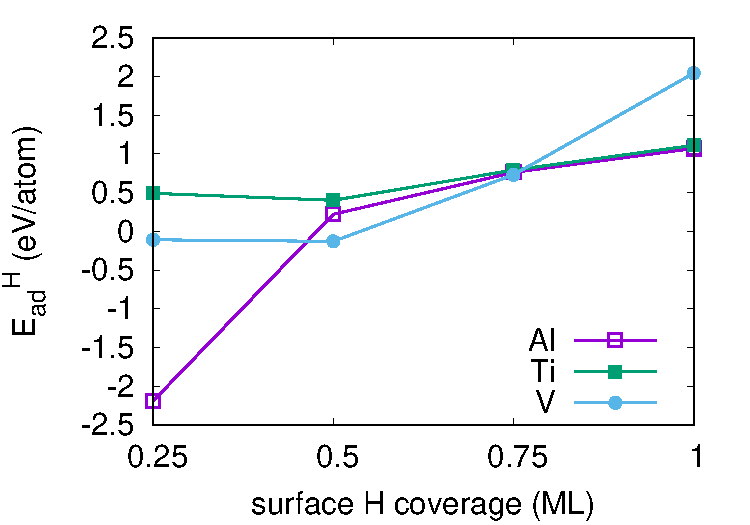
\includegraphics[width=0.4\linewidth]{Chap1/plots/E_C_1.pdf}}\label{Chap:ZnO_H:fig:dop1}
  \subfigure[]{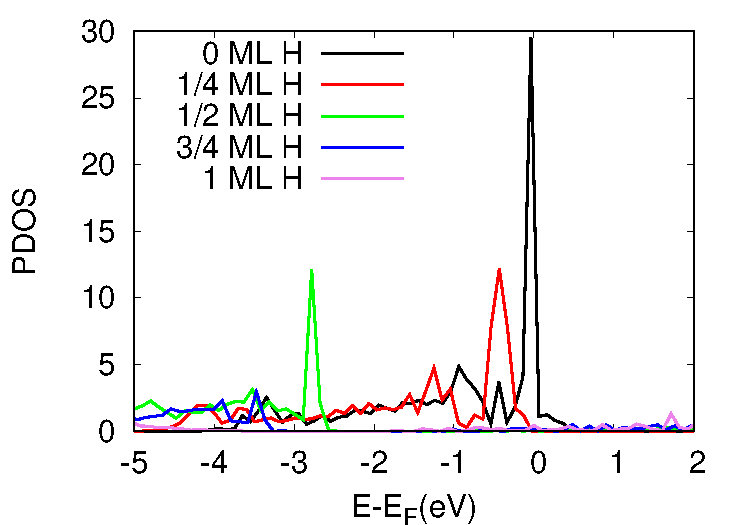
\includegraphics[width=0.4\linewidth]{Chap1/plots/DOS_Al_surfO.pdf}}\label{Chap:ZnO_H:fig:dop2}
  \\
  \subfigure[]{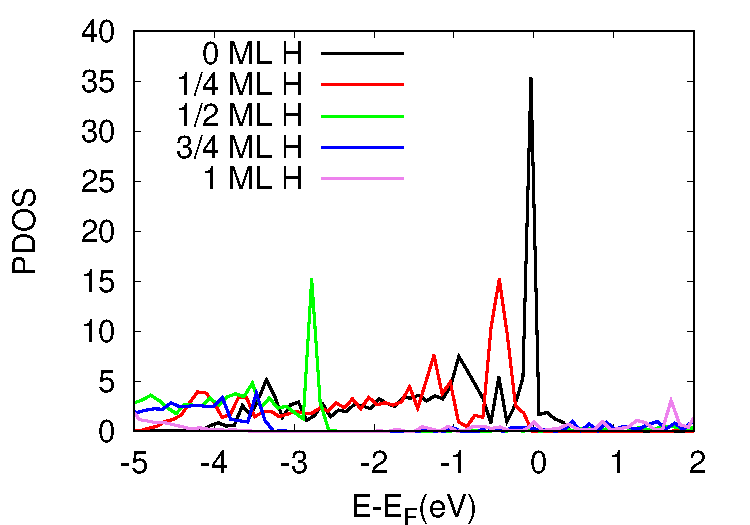
\includegraphics[width=0.4\linewidth]{Chap1/plots/DOS_Al_surf_all.pdf}}\label{Chap:ZnO_H:fig:dop3}
  \subfigure[]{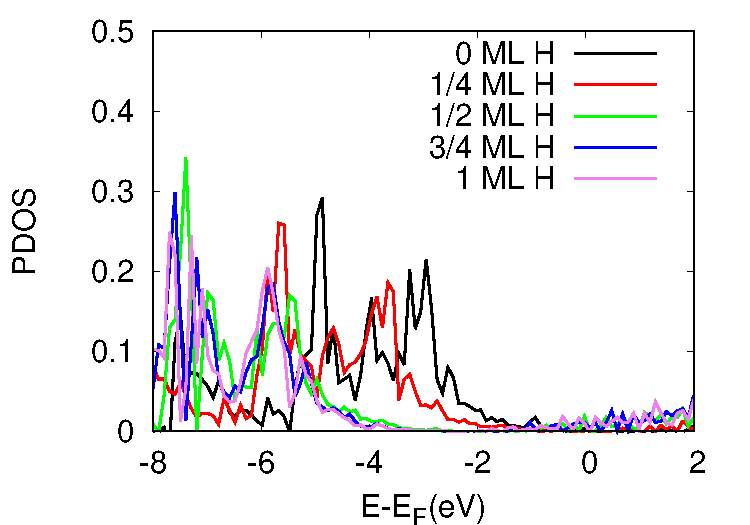
\includegraphics[width=0.4\linewidth]{Chap1/plots/DOS_bulk_Al.pdf}}\label{Chap:ZnO_H:fig:dop4}
  \\
  \subfigure[]{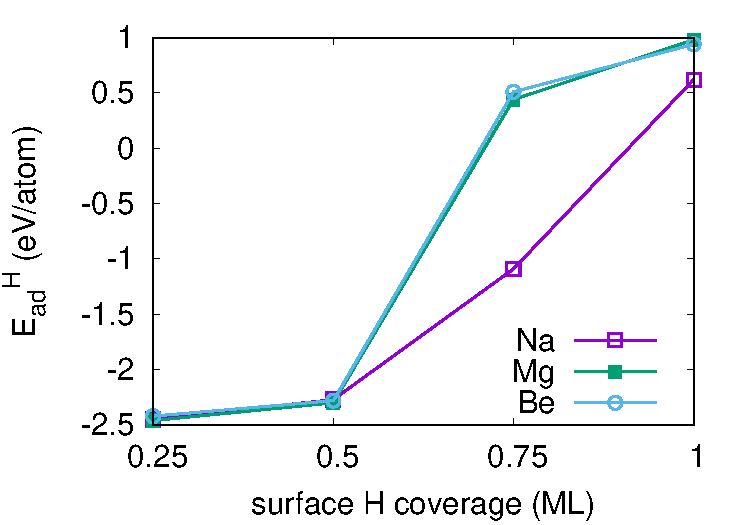
\includegraphics[width=0.4\linewidth]{Chap1/plots/E_C_2.pdf}}\label{Chap:ZnO_H:fig:dop5}
  \subfigure[]{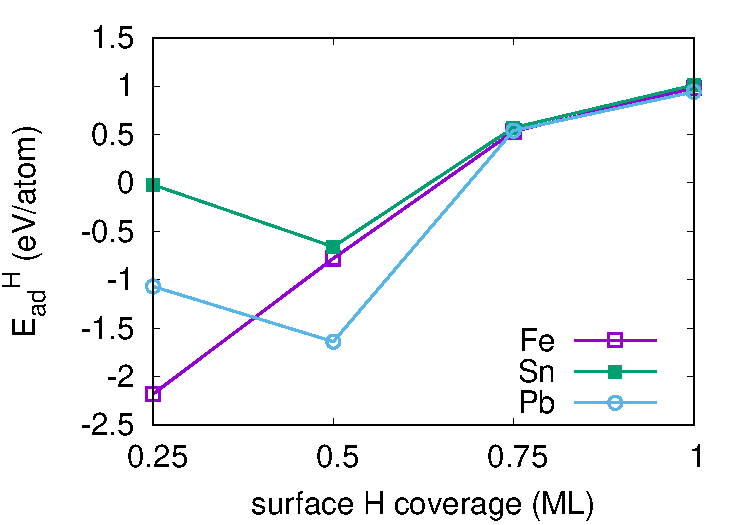
\includegraphics[width=0.4\linewidth]{Chap1/plots/E_C_3.pdf}}\label{Chap:ZnO_H:fig:dop6}
\caption[H adsorptions on ZnO surfaces with different doping]{(a)$E_{\textup{ad}}^{\textup{H}}$ on (2$\times$2) ZnO (000$\overline{1}$) surface with one substitutional dopant atom at Zn site. Each dopant atom has more valence electrons more than Zn. (b)\ac{PDOS} for all the O atoms on top surface layer of Al-doped ZnO (000$\overline{1}$) under different $\theta_{\textup{H}}$. (c)\ac{PDOS} of all O, Zn and adsorbed H atoms on the topmost layer of Al-doped ZnO (000$\overline{1}$) under different $\theta_{\textup{H}}$. (d)\ac{PDOS} for Al atom in the bulk layer of Al-doped ZnO (000$\overline{1}$) under different $\theta_{\textup{H}}$. (e)$E_{\textup{ad}}^{\textup{H}}$ on (2$\times$2) ZnO(000$\overline{1}$) surface with one substitutional dopant atom at bulk Zn sites. Each dopant atom has equal or less valence electrons than Zn. (f)$E_{\textup{ad}}^{\textup{H}}$ on (2$\times$2) ZnO(000$\overline{1}$) surface with one substitutional dopant atom at bulk Zn sites. Each dopant atom has multiple common charge states.}
\label{Chap:ZnO_H:fig:doped}
\end{figure}
\endgroup

The dopant atoms located at slab layers with different distances to the top (000$\overline{1}$) surface layer are investigated, and our results show that the location of such dopant atom does not have a significant effect on H adsorption energetics and the critical $\theta_{\textup{H}}$. As illustrated in Tab. \ref{tab:layer}, H adsorption energies with the substitutional dopant elements on Zn lattice sites at different layers away from the O-terminated (000$\bar{1}$) surfaces are listed. H adsorption energies do not show significant variations for the dopant atom at varying distances to the top layer of (000$\bar{1}$) surfaces. Thus, the results for one dopant atom (Al, Ti, V, Na, Mg, Be, Fe, Sn, and Pb) at bulk Zn site far away from the top surface layer in (2$\times$2) ZnO (000$\overline{1}$) supercells are summarized in Fig. \ref{Chap:ZnO_H:fig:doped}. 

\begin{table}[!htbp]
\centering
\caption[Comparison of different doping locations to the top surface layer]{The coverage-dependent adsorption energy of H atom $E_{\textup{ad}}^{\textup{H}}$ (unit: eV/atom) on O-terminated  (000$\bar{1}$) ZnO surface with substitutional Be dopant atom at different locations to the top surface layer. Layer 1 is at the Zn lattice site nearest to the top surface layer.}
\label{tab:layer}
\begin{tabular}{lllll}
\\
\hline
\hline
eV/atom      & 0.25ML & 0.5ML & 0.75ML & 1ML  \\ \hline
Layer 1      & -2.71  & -2.39 & 0.52   & 0.97 \\
Layer 2      & -2.38  & -2.23 & 0.43   & 0.97 \\
Layer 3      & -2.42  & -2.28 & 0.51   & 0.94 \\
Layer 4      & -2.39  & -2.32 & 0.46   & 0.98 \\
\hline
\hline
\end{tabular}
\end{table}

In Fig. \ref{Chap:ZnO_H:fig:dop1}, all dopant atoms (Al, Ti and V) have more valence electrons than Zn. For Al-doped ZnO surface, if the one extra valence electron from Al already transfers to O atoms on the top surface layer, only one H atom is required to saturate all 4 O atoms in a (2$\times$2) supercell and induce the metal-semiconductor transition according to the electron counting model. Consistent with this interpretation, the H adsorption strength for the Al-doped ZnO surface in Fig. \ref{Chap:ZnO_H:fig:dop1} is as strong as the pure ZnO surface in Fig. \ref{Chap:ZnO_H:fig:Ead} when $\theta_{\textup{H}}$ $\leq$ $\frac{1}{4}$ ML. Above this critical $\theta_{\textup{H}}$, $E_{\textup{ad}}^{\textup{H}}$ suddenly increases to positive values, consistent with the proposed metal-semiconductor transition for ZnO surface. This interpretation is further confirmed by analyses of \acf{PDOS} of all four surface O atoms on (2$\times$2) Al-doped ZnO surface in Fig. \ref{Chap:ZnO_H:fig:dop2}. \ac{PDOS} of O atoms with $\theta_{\textup{H}}$ = 0 ML case have strong peaks at the Fermi level. When Al-doped ZnO surfaces are covered by $\frac{1}{4}$ to 1 ML of H atoms, there are no peaks on the Fermi level, making these surfaces in semiconductor states. \ac{PDOS} of all surface atoms, including all the O, Zn and adsorbed H atoms on the topmost layer of Al-doped ZnO (000$\overline{1}$) surface, are plotted in Fig. \ref{Chap:ZnO_H:fig:dop3} to confirm the above analyses. Similar to Fig. \ref{Chap:ZnO_H:fig:dop2},  \ac{PDOS} of all surface atoms for the case of $\theta_{\textup{H}}$ =  0 ML  show strong peaks in the Fermi level, while \ac{PDOS} of all surface atoms for the cases of $\theta_{\textup{H}}=\frac{1}{4}$ ML and above exhibit semiconductor characteristics. \ac{PDOS} of the Al atom, which is located at the third layer away from the (000$\overline{1}$) O-term surface, under different H surface coverages is also plotted in Fig. \ref{Chap:ZnO_H:fig:dop4}.  As can be seen from the plot, there is no significant peak around Fermi level for all the H surface coverages, showing that the bulk Al atom under different H surface coverages is also saturated in closed-shell electron configuration. Interestingly, \ac{PDOS} of Al downshifts indicating a stronger bonding between Al and nearby O atoms as the H surface coverages increases.

If one Zn atom is replaced by one Ti or V atom in the (2$\times$2) supercell, because both Ti and V have two or more valence electrons than Zn, all O atoms on (000$\overline{1}$) surface are already saturated without any adsorbed H atoms. Therefore,  both Ti-doped and V-doped ZnO surfaces have very weak H adsorption strengths with $E_{\textup{ad}}^{\textup{H}}$ close to or above zero for all $\theta_{\textup{H}}$ values in Fig. \ref{Chap:ZnO_H:fig:dop1}. Meanwhile, if one Zn atom is replaced by one dopant atom with two valence electrons the same as Zn, such as beryllium (Be) or magnesium (Mg), the variations of $E_{\textup{ad}}^{\textup{H}}$ with $\theta_{\textup{H}}$ are almost the same as those on pure ZnO surface as shown in Fig. \ref{Chap:ZnO_H:fig:dop5}, so the doped ZnO (000$\overline{1}$) surfaces have strong H adsorption strength only when $\theta_{\textup{H}}$ $\leq$ $\frac{1}{2}$ ML. If one Zn atom is replaced by a dopant atom with only one valence electron such as sodium (Na), the dopant can attract one electron from O atoms on (2$\times$2)  (000$\overline{1}$) surface, so three H atoms are required to saturate all 4 O atoms in a (2$\times$2) supercell. Correspondingly, this Na-doped ZnO (000$\overline{1}$) surface has strong H adsorption strength when $\theta_{\textup{H}}$ $\leq$ $\frac{3}{4}$ ML  as shown in Fig. \ref{Chap:ZnO_H:fig:dop5}. 

Moreover, the dopant effects of elements with multiple common charge states are shown in Fig. \ref{Chap:ZnO_H:fig:dop6}. Fe has both +2 and +3 charge states, so the Fe-doped ZnO (000$\overline{1}$) shows H adsorption strengths at the intermediate level between those on Mg-doped and Al-doped ZnO (000$\overline{1}$) surfaces. It only demonstrates strong H adsorption strengths ($E_{\textup{ad}}^{\textup{H}}$ $\ll$ 0 ) only when $\theta_{\textup{H}}$ $\leq$ $\frac{1}{2}$ ML, similar to the cases for Mg dopant, but the adsorption energy of the second H atom ($\theta_{\textup{H}}$ = $\frac{1}{2}$ ML) is much weaker than that of pure ZnO,  similar to the cases for Al dopant. Meanwhile, Sn and Pb elements can have variant charge states ranging from +1 to +4, with +2 and +4 as the most common states\cite{Greenwood97}. Because of the +2 charge state, ZnO (000$\overline{1}$) with either a Sn or Pb dopant atom show very weak H adsorption strengths ($E_{\textup{ad}}^{\textup{H}}$ $\gg$ 0 ) when $\theta_{\textup{H}}$ $>$ $\frac{1}{2}$ ML, similar to the cases for Mg dopant.  However, since each Sn or Pb atom can contribute more than 2 electrons to ZnO (000$\overline{1}$) surface, H adsorption strengths are also significantly weakened when $\theta_{\textup{H}}$ $\leq$ $\frac{1}{2}$ M. In addition, because the +3 charge state is not as stable as +2 or +4 states for Sn/Pb\cite{Greenwood97}, $E_{\textup{ad}}^{\textup{H}}$ of the first H atom ($\theta_{\textup{H}}$ = $\frac{1}{4}$ ML) is even weaker (more positive) than $E_{\textup{ad}}^{\textup{H}}$ of the second H atom ($\theta_{\textup{H}}$ = $\frac{1}{2}$ ML).